This section dives into the details of the modified Firefly-Gossip Protocol (FiGo)  protocol, responsible for synchronizing both clocks and payload data. We will formally describe the deviation of internal clock ticks. Additionally, we will present the algorithm used for clock computation and synchronization at the network edge. To lay the groundwork, we first formalize the architectural and behavioral language of OMNeT++, allowing us to capture the system's architecture accurately.

\subsection{Formalization of OMNeT++}
\includesection{omnet}


The purpose of verifying FiGo protocol is to ensure that liveness and safety requirements. In the context of the FiGo protocol, the liveness requirement is expressed as follows: \quot{\emph{When the clock ticks of the sensors are not synchronized, they should eventually synchronize}}. In the payload case, the liveness requirement is expressed as follows: \quot{\emph{When the sensor payloads are not equivalent, they should eventually become equivalent.}} However, the safety requirement ensures that \quot{\emph{the sensor command is received at the same instant of time H}}.

\subsection{The Firefly-Gossip Protocol}

The FiGo algorithm has been specifically implemented for object synchronization, as demonstrated in \cite{WEBSTER2020101183, WebsterBDFM18, Oxford2020}. However, researchers have made modifications to fine-tune the algorithm to meet their specific requirements. Initially, the algorithm was designed to synchronize clocks among sensor nodes (\fig{fig:edge}), facilitating a unified time measurement across the network. Our modifications to the algorithm enable the edge gateway to calculate the average clock of the sensor nodes. The modified algorithm is presented in Algorithm \ref{algo:model:algo:figo}. Input parameters include \texttt{cycleLength}, \texttt{refractoryPeriod}, the \texttt{nextBroadcast}, and \texttt{sameThreshold}. The \texttt{refractoryPeriod} is a duration during which no further transmissions are made after the initial transmission to conserve energy usage. The \texttt{cycleLength} is the total period in which the sensor node is performing computation, transmission, and sleeping (i.e.,  \texttt{refractoryPeriod}). The \texttt{nextBroadcast} represents the precise moment in time when the sensor node transmits its local clocks and payload.

\noindent
\begin{figure}[!htbp]
    \centering
    		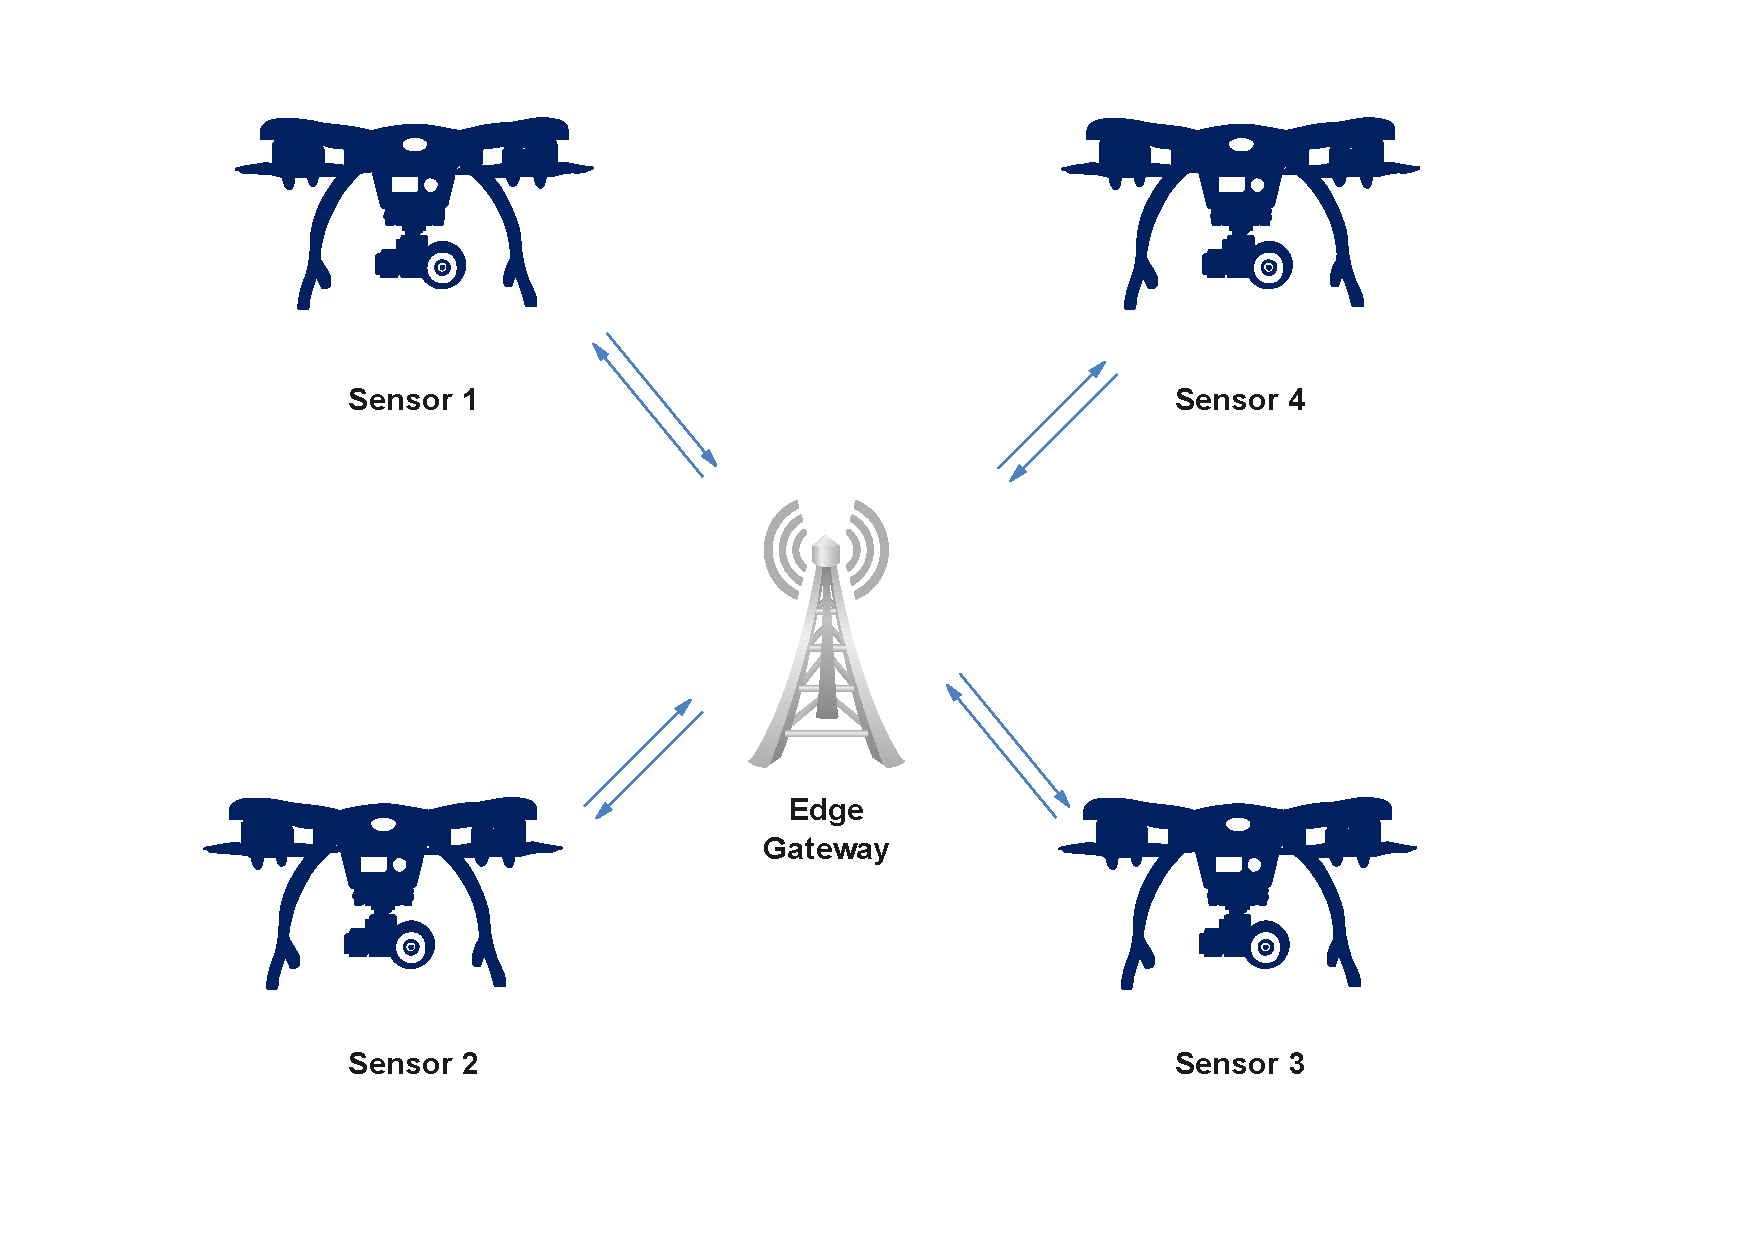
\includegraphics[width=250pt, height =150pt]{exampleEdge.pdf}
    \caption{Sensor Nodes Orchestration using Edge Gateway. }
    \label{fig:edge}
\end{figure} 


Each sensor node is uniquely identified by its local clock tick \texttt{H}, payload \texttt{Pld}, and the collected message \texttt{msg}, which is initially empty. Additionally, the \texttt{sameCount} flag is used to indicate the number of times the message has been broadcasted out of the sensor nodes zone. These sensor information are portrayed in lines 1-4. 

In the initial stage of the protocol, in line 6, the sensor node actively listens for incoming messages. If the message is stated \texttt{listening} (line 7), the protocol is triggered to execute the instructions outlined in lines 8-26. if the sensor node is in sleeping mode, then it calibrates its clocks to the average value of the sensor nodes of its zones gathered from the zone gateway (lines 8-11). If the collected payload and the sensor payload are equivalent, the sensor node sends an order to the activator and increments the \texttt{sameCount} value to 1, indicating that one order has been executed during the \texttt{cycleLength}. If the sensor payload exceeds the calculated average, it needs to be calibrated.
Similarly, if the payload differs from the message payload, the sensor should transmit its information to the gateway to recalculate the average time value. This operation is executed when the sensor nodes disconnect from the sensor zone. Furthermore, if the received message is not in the listening mode, a broadcast is sent to the gateway, and the \texttt{sameCount} is reset.


When a sensor's \texttt{cycleLength} is reached, both the local clock tick and the \texttt{sameCount} are reset in lines 29-30. When the sensor clock tick does not meet the sensor's \texttt{cycleLength}, the sensor clock tick continues to increase.

\RestyleAlgo{ruled}

%% This is needed if you want to add comments in
%% your algorithm with \Comment
\SetKwComment{Comment}{\gtext{/*} }{ \gtext{*/}}
\begin{algorithm}[H]
\label{algo:model:algo:figo}
\caption{FiGo Communication and Synchronization Protocol}
%\caption{An algorithm with caption}\label{alg:two}
\KwData{cycleLength, refractoryPeriod, nextBroadcast, sameThreshold.}
$H \gets Init$ \Comment*[r]{\gtext{The initial value of drone tick.}}
$Pld \gets 1$ \Comment*[r]{\gtext{The initial payload value.}}
$msg \gets empty()$ \Comment*[r]{\gtext{The message status.}}
$sameCount \gets 0$ \Comment*[r]{\gtext{The same count variable for lifting.}}
\While{$True$}{
    $msg\gets heard();$ \\
    \eIf{$msg.listen()$}{

         \If{($H \ > \ refractoryPeriod$)}
        { $H  \gets  msg.H$\Comment*[r]{\gtext{Update the local clock tick with the synchronized tick.}}
          $Pld  \gets  msg.Pld;$\\
        }
        
              \eIf{($Pld$ == $msg.Pld$)}{
                    $sameCount \gets sameCount+1;$\\
                    $sendCommand(H,Pld)$\Comment*[r]{\gtext{Send lift message to the crane.}}
                    $Pld  \gets sensing()$\Comment*[r]{\gtext{Sensing a new payload.}}
                }{
                    \eIf{($Pld$ > $msg.Pld$)}{
                        $Pld  \gets  msg.Pld$\\ 
                    }{
                        $transmit(H, Pld)$  
                    }
                }
        }
    { 
     \If{(H==nextBroadcast) || ( (H==(nextBroadcast+refractoryPeriod) \% cycleLenght) \&\& sameCount<sameThreshold)}
     {
        $transmit(H, Pld)$\Comment*[r]{\gtext{transmits the local clock tick and payload to the gateway.}}
        $sameCount\gets0;$
     }
    }

    \eIf{($H$==$cycleLenght$)}
    { $H\gets 0$ \Comment*[r]{\gtext{reset the clock tick and sameCount.}}
      $sameCount \gets 0$;
    }
    {
     $H\gets H+1$ \Comment*[r]{\gtext{tick progress until cycle length is reached.}}
    }
}
\end{algorithm}


\subsection{Clock Deviation in FiGo}
In the absence of synchronization, device clocks operate autonomously without coordination. Each sensor sends its payload at its own clock frequency without acknowledging a reference clock. Taking into account the implementation of the FiGo protocol outlined in Algorithm \ref{algo:model:algo:figo}, the clock progress is carried out by the sensor at \cmt{line 33}, utilizing a one-time unit. However, in the presence of environmental conditions, the internal clock ticks may progress differently. It is assumed that in the presence of drifting, the clock progress occurs with an interval of two-time units \cite{WEBSTER2020101183}. In the background section, we \cmt{have introduced} three distinct approaches to illustrate progress with different rates. Assuming that the rate of drift is denoted as \emath{\lambda}, we model two rules inherited from OMNeT++ \ref{eq1} as follows:

\noindent

\begin{boxD}
%\framedtext{

   \begin{equation}\frac{ s_{0} \gparrow{\tau}_{\lambda} s'_{0}} { \langle s_{0},\ldots,s_{n},X\rangle \xrightarrow{\tau}_{\lambda}\langle s'_{0},\ldots,s_{n},X'\rangle  } \label{eqc1} \tag{\emph{Clock Drift}} 
   \end{equation}
      where  \emath{X'_{H_{l}}=X[H_{l}:=H_{l}+2]} 

         \begin{equation}\frac{ s_{0} \gparrow{\tau}_{1-\lambda} s'_{0}} { \langle s_{0},\ldots,s_{n},X\rangle \xrightarrow{\tau}_{1-\lambda}\langle s'_{0},\ldots,s_{n},X'\rangle  } \label{eqc2} \tag{\emph{No Clock Drift}} 
   \end{equation}
      where  \emath{X'_{H_{l}}=X[H_{l}:=H_{l}+1]} 
	     
\end{boxD}

\RestyleAlgo{ruled}

\subsection{The Synchronization Gateway}
Clock drift mitigation involves the utilization of an intermediary component or coordinator to reset the internal clock. This reset is based on the average of the clocks received from various devices, as emphasized by \cite{WebsterBDFM18}. In our proposed approach, the coordinator is responsible for gathering the internal clocks from all the sensors. Once the clocks are collected, an averaging calculation is performed to determine the new clock value. Subsequently, this new value is communicated back to the respective devices.


The classical FiGo algorithm handles synchronization among the sensor nodes. However, in this modified version, the responsibility for synchronization is shifted to the gateway. When a sensor transmits its local clock and payloads, the gateway performs the synchronization process. For this purpose, we refer to the gateway as \quot{InBox}. The algorithm depicting this synchronization process can be found in Algorithm \ref{algo:model:algo:inbox}.

Algorithm \ref{algo:model:algo:inbox} is designed to operate with the maximum sensor value, denoted as \texttt{max}, within its designated area. Each gateway is uniquely identified in lines 1-6 based on its calculated clock tick \texttt{H}, payload \texttt{Pld}, and the received/sent message \texttt{msg}. The variable \texttt{Length} represents the count of received transmit messages and is initialized to 0. The payload and clock ticks are stored separately in two distinct stacks, namely \texttt{ListOfH} and \texttt{ListOfPld}.

The \quot{InBox} gateway initiates the process by listening to incoming messages, as indicated in line 8 of the algorithm. If the message is flagged as being in transmit mode, the corresponding clock tick and payload are pushed into their respective stacks, namely \texttt{ListOfH} and \texttt{ListOfPld} in lines 10-11. In this algorithm, the length is incremented to keep track of the received messages. When the length of received messages reaches the maximum number of incoming messages (i.e., sensor nodes), the gateway calculates the average clock ticks and payload in lines 15-16. Subsequently, it broadcasts these messages to its neighboring nodes in line 17. Finally, the stack length is reset to 0, and the stacks are emptied. Formally, we model the operational semantics of the messages received (including clocks and payloads) by the inbox originating from sensor nodes using Rule \ref{eqs1}. On the other hand, Rule \ref{eqs2} describes how the averaged clock is broadcasted to the sensor nodes. The communication channel selected for data transfer is denoted as \quot{p}.


\begin{boxD}
%\framedtext{

   \begin{equation}\frac{ s_{0} \gparrow{p?\langle H, Pld\rangle} s'_{0}} { \langle s_{0},\ldots,s_{n},X\rangle \xrightarrow{p}\langle s'_{0},\ldots,s_{n},X'\rangle  } \label{eqs1} \tag{\emph{Receive}} 
   \end{equation}
      where  \emath{X'=X[length:=length+1]} 

         \begin{equation}\frac{ \sset{Inbox} =s_{i} \gparrow{p!\langle H, Pld\rangle} s'_{i} \bigwedge_{j \ldots n} \sset{\mathcal{ND}_{j}} =s_{j} \gparrow{p?\langle H, Pld\rangle} s'_{j}} { \langle s_{i}, s_{j},\ldots,s_{n},X\rangle \xrightarrow{p}\langle s'_{i},s'_{j},\ldots,s_{n},X'\rangle  } \label{eqs2} \tag{\emph{Broadcast}} 
   \end{equation}
      where  \emath{X'=X[length:=0]} 
	     
\end{boxD}

%% This is needed if you want to add comments in
%% your algorithm with \Comment
\SetKwComment{Comment}{\gtext{/*} }{ \gtext{*/}}
\begin{algorithm}[H]
\label{algo:model:algo:inbox}
\caption{InBox implementation at the Edge Gateway}
%\caption{An algorithm with caption}\label{alg:two}
\KwData{max.}
$H \gets Init$ \Comment*[r]{\gtext{The initial value of drone tick.}}
$Pld \gets 1$ \Comment*[r]{\gtext{The payload message for crane lifting.}}
$msg \gets empty()$ \Comment*[r]{\gtext{The message status.}}
$Length \gets 0$ \Comment*[r]{\gtext{The drones length.}}
$ListOfH \gets stack()$ \Comment*[r]{\gtext{The list of clock ticks.}}
$ListOfPld \gets stack()$ \Comment*[r]{\gtext{The list of payload.}}
\While{$True$}{
    $msg\gets heard();$ \\
    \If{($msg.transmit()$)}{
    $ListOfH.push(msg.H)$ \Comment*[r]{\gtext{push the received clock ticks to the stack.}}
    $ListOfPld.push(msg.Pld)$ \Comment*[r]{\gtext{push the received payloads to the stack.}}
    $Length \gets Length +1$ \Comment*[r]{\gtext{increments the stack length.}}
    }
    \If{($Length == max$)}{ 
     $H \gets \text{AVG}(ListOfH)$ ;\\
     $Pld \gets \text{AVG}(ListOfPld)$ ;\\
     $broadcast( H, Pld )$ \Comment*[r]{\gtext{broadcast the average value of clock ticks and payloads.}}
      $Length \gets 0$\\
      $ListOfH \gets empty()$\\
      $ListOfPld \gets empty()$\\
    }
    
    
}
\end{algorithm}

